\chapter{Einleitung}\label{einleitung}

\section{Vorstellung der \webco}
Die \webco besteht seit dem Jahr 1999 in Form eines eigenständiges Unternehmens als Full-Service-Internet-Dienstleister. Die Haupttätigkeit der etwa 20 Mitarbeiter besteht in der kontinuierlichen Neu- und Weiterentwicklung von maßgeschneiderten Internet-Anwendungen nach den persönlichen Kundenwünschen. Die Entwicklung des eigenen \cms (kurz \cms) \edith begann mit der Firmengründung und wird fortlaufend weiterentwickelt. Auf der Basis von dem \cmsEdith\, läuft das Projekt \qmUO{\sesam}. 
\abschnitt
Das auf \edith-basierte Projekt \qmUO{\sesam} ist ein Baukasten für die Erstellung eigener Webseiten in den Seelsorgeeinheiten der Erzdiözese Freiburg. Neben den Seelsorgeeinheiten nutzen auch Dekanate, Diözese-Anstellen und sonstige Einrichtungen das System.
\abschnitt
Neben dem eigenen \cmsEdith\, wird je nach Projektumfang und -anforderungen das Open-Source \cms TYPO3 eingesetzt.


\section{Problemstellung} \label{problemstellung}
Mit dem Projekt \qmUO{Sesam} unterstützt das Erzbischöfliche Ordinariat Freiburg seine Einrichtung bei der Realisierung eines Internet-Auftrittes. Zum Einsatz kommt das von \webco entwickelte \cmsEdith, welches von derzeit ca. 500 SESAM-Mandanten genutzt wird.
\abschnitt
Ein großer Teil dieser Mandanten verwaltet mit \edith\, die Gottesdienst-Termine und gibt diese auf dem eigenen Internetauftritt aus. Bei vielen werden die verwalteten Termindaten in den individuell gestalteten Pfarrbriefen oder Gemeindebriefen verwendet.

\exkurs{Pfarrbrief}{Als Pfarrbrief oder Gemeindebrief wird ein Heft verstanden, das eine christliche Gemeinde als Informationsmedium periodisch an die Mitglieder der Kirche her ausgibt. Oft bildet ein Grußwort eines Pfarrers oder ein geistlicher Impuls den Beginn. Nachfolgend werden Bericht oder Ankündigungen aus der Gemeindearbeit aufgeführt. Abschließend folgt ein Veranstaltungskalender.}

Bislang steht für die Generierung des individuellen Pfarrbriefes eine sehr einfach gehaltene Export-Funktion zur Verfügung, die jedoch nur wenig Gestaltungsmöglichkeiten bietet. Demgegenüber stehen zahlreiche Pfarrbriefvarianten, die sich hinsichtlich Struktur und Formatierung teilweise erheblich unterschieden.
\abschnitt
Um diese Vielfältigkeit der Pfarrbriefe zu verdeutlichen befinden sich in Abbildung \ref{img:Gemeindebrief} zwei unterschiedliche aussehende Pfarrbriefe.\newline
\begin{figure}[h]
    \caption{Pfarrbriefe}
    \label{img:Gemeindebrief}
        \subfigure[Gottesdienste Juli – August 2017 – Katholische Kirche an der Schutter \cite{KatholischeKirchengemeindeanderSchutter.2017}]{
            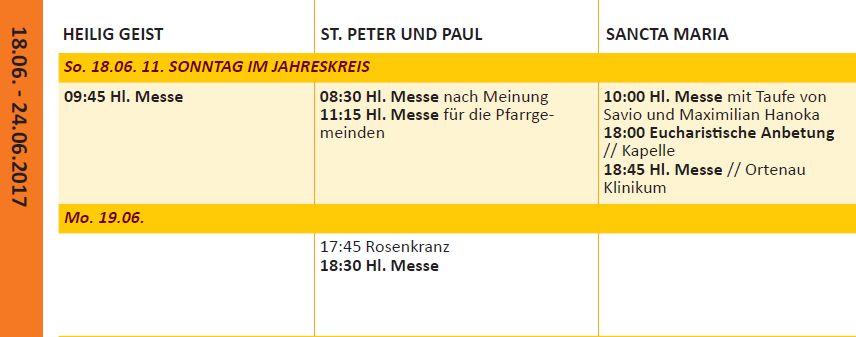
\includegraphics[width=8 cm]{bilder/Gemeindebrief_Schutter.png}
            \label{img:PfarrbriefSchutter} }
        \subfigure[Gemeindebrief vom Mai 2018 – Baden-Baden \cite{Kath.KirchengemeindeBadenBaden.2017}]{
        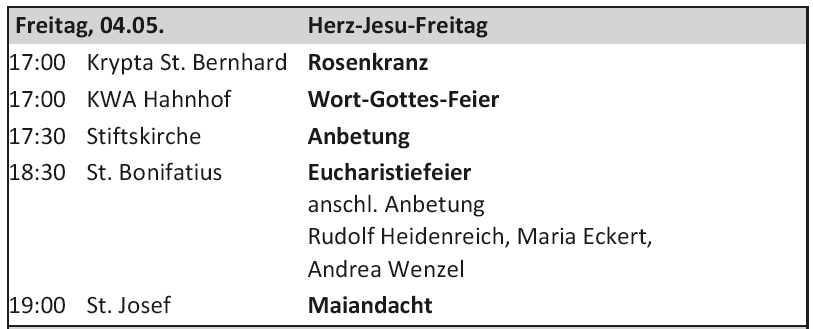
\includegraphics[width=8 cm]{bilder/Gemeindebrief_BadenBaden.png}
        \label{img:PfarrbriefBadenBaden} }
\end{figure}\newline
Sofort ist zu erkennen, dass sich die Pfarrbriefe nicht nur in den Farbe unterscheiden, sondern auch in der Form. Im Pfarrbrief von der Katholischen Kirche an der Schutter, Abbildung \ref{img:PfarrbriefSchutter}, werden die verschiedenen Gottesdienste zuerst auf die verschiedenen Kirchen aufgeteilt und dann den entsprechenden Tagen eingeteilt. Im Gemeindebrief von Baden-Baden, Abbildung\ref{img:PfarrbriefBadenBaden}, hingegen werden die Gottesdienste den Tagen zugeteilt und dann die jeweiligen Kirche einer einzelnen Veranstaltung.
\abschnitt
Um diesen individuellen Ansprüchen der Pfarrblatt-Gestaltung gerecht zu werden, muss das Export-Ergebnis daher manuell aufwändig nach bearbeitet werden. Dafür werden in der Regel die Programme Microsoft Word, Microsoft Publisher oder Adobe InDesign eingesetzt.
\abschnitt
Die mühselige Nacharbeitung erfolgte durch einen nicht technisch begabten Angestellten oder ehrenamtlichen Nutzer der Institutionen mithilfe von \qmUO{Copy \& Paste} in die bevorzugte Software in das gewünschte Design. Die Abbildung \ref{img:AblaufErstellungPfarrbrief} zeigt nochmal den Ablauf für die Erstellung eines Pfarrbriefes. Für diese Arbeit ist der Ablauf im \cmsEdith \, und in der bevorzugten Software, Microsoft Word, Microsoft Publisher oder Adobe InDesign essentiell. An diesen Abschnitten der Erstellung soll eine Verbesserung erfolgen.\newline
\begin{figure}[h]
	\centering
	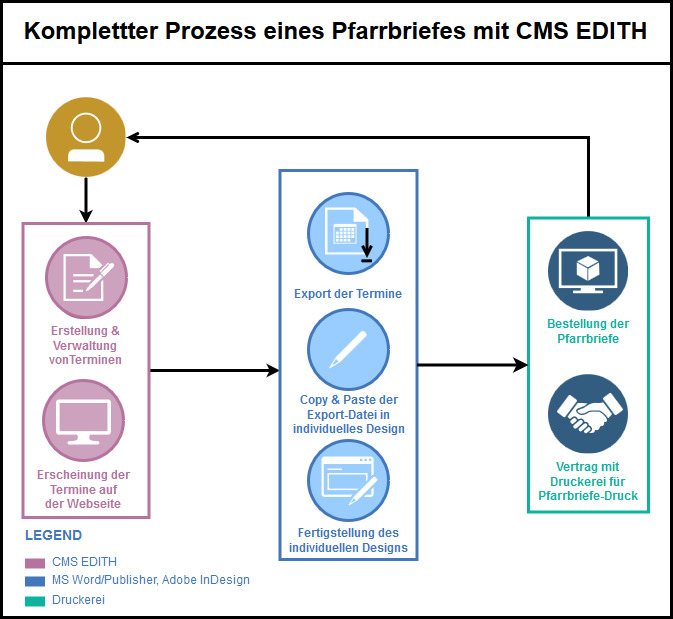
\includegraphics[width=12cm]{bilder/kompletterJetzigerProzess.png}
    \caption{Auflauf zur Erstellung eines Pfarrbriefes mit der bisherigen Export-Funktion}
    \label{img:AblaufErstellungPfarrbrief}
\end{figure} \abschnitt

\section{Motivation} \label{motivation}



\section{Zielsetzung} \label{zielsetzung}
Im Rahmen der Bachelorarbeit soll eine neue Export-Funktion konzipiert werden und in Form eines Prototyps umgesetzt werden. Der Export soll dabei eine möglichst individuelle Ausgabe der Termindaten ermöglichen, sodass deutlich weniger Nachbearbeitungsaufwand für die Mitarbeiter und Mitarbeiterinnen der kirchlichen Einrichtungen anfällt. Im Rahmen der Projektarbeit 3 wurden bereits die Anforderungen an einen solchen Export ermittelt und eine Machbarkeitsanalyse durchgeführt. Es stellt sich dabei heraus, dass das Dateiformat \qmUO{DOCX} in diesem Anwendungskontext sehr gut eignet. \abschnitt
Nach der Fertigstellung des Prototypen soll anhand von den erstellten Anforderungen und Metriken der Prototyp evaluiert werden. So kann festgestellt werden, ob der Prototyp in die Umgebung des \cmsEdith \, integriert werden kann.


\section{Vorgehensweise} \label{vorgehensweise}
